\documentclass[../main.tex]{subfile}

\begin{document}

\begin{figure}
    \centering
    \subfloat[Class A]{
        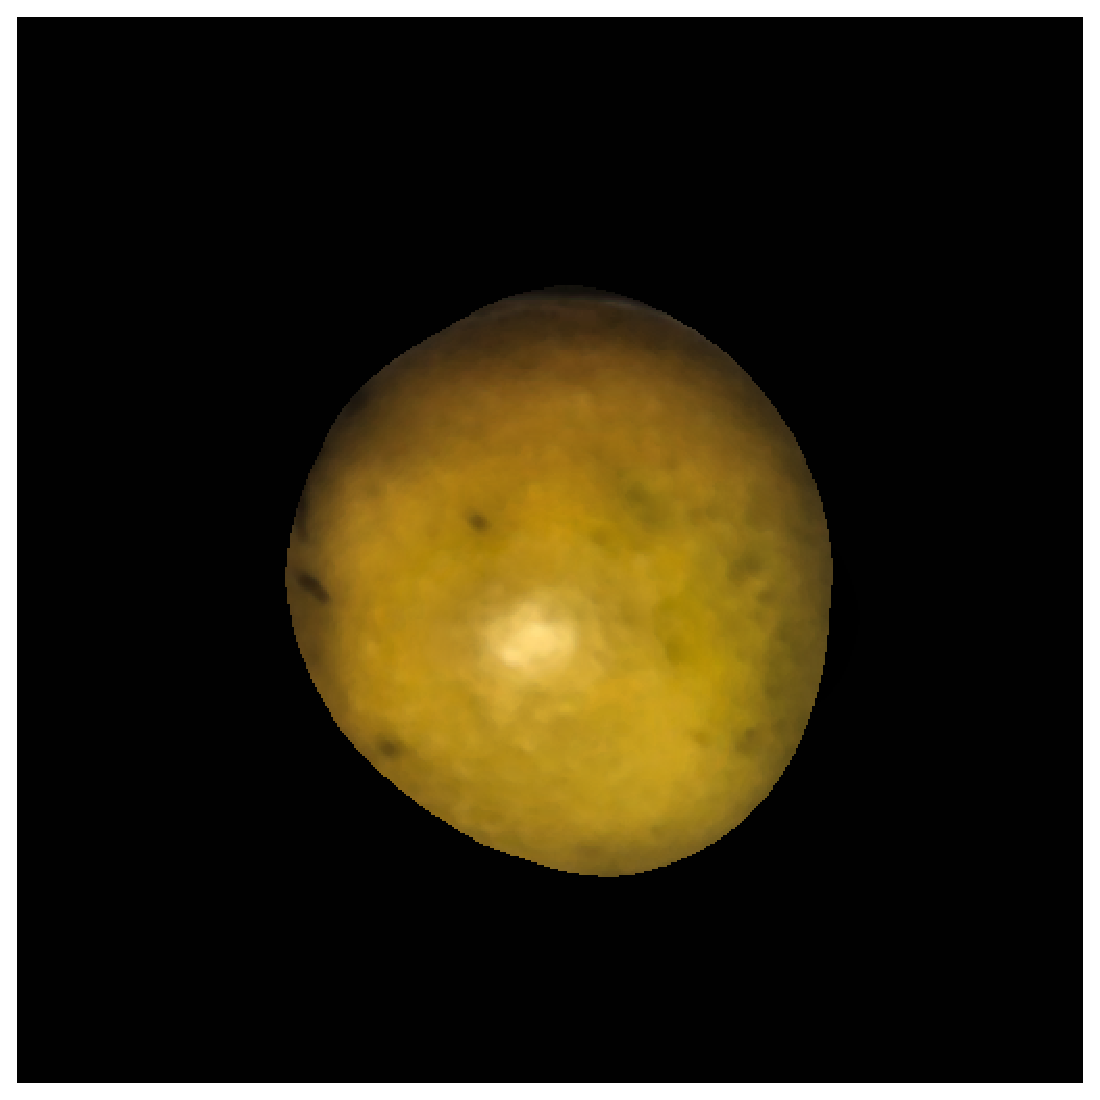
\includegraphics[width=.15\textwidth]{images/classes/abiu-good.eps}
    }
    \subfloat[Class B]{
        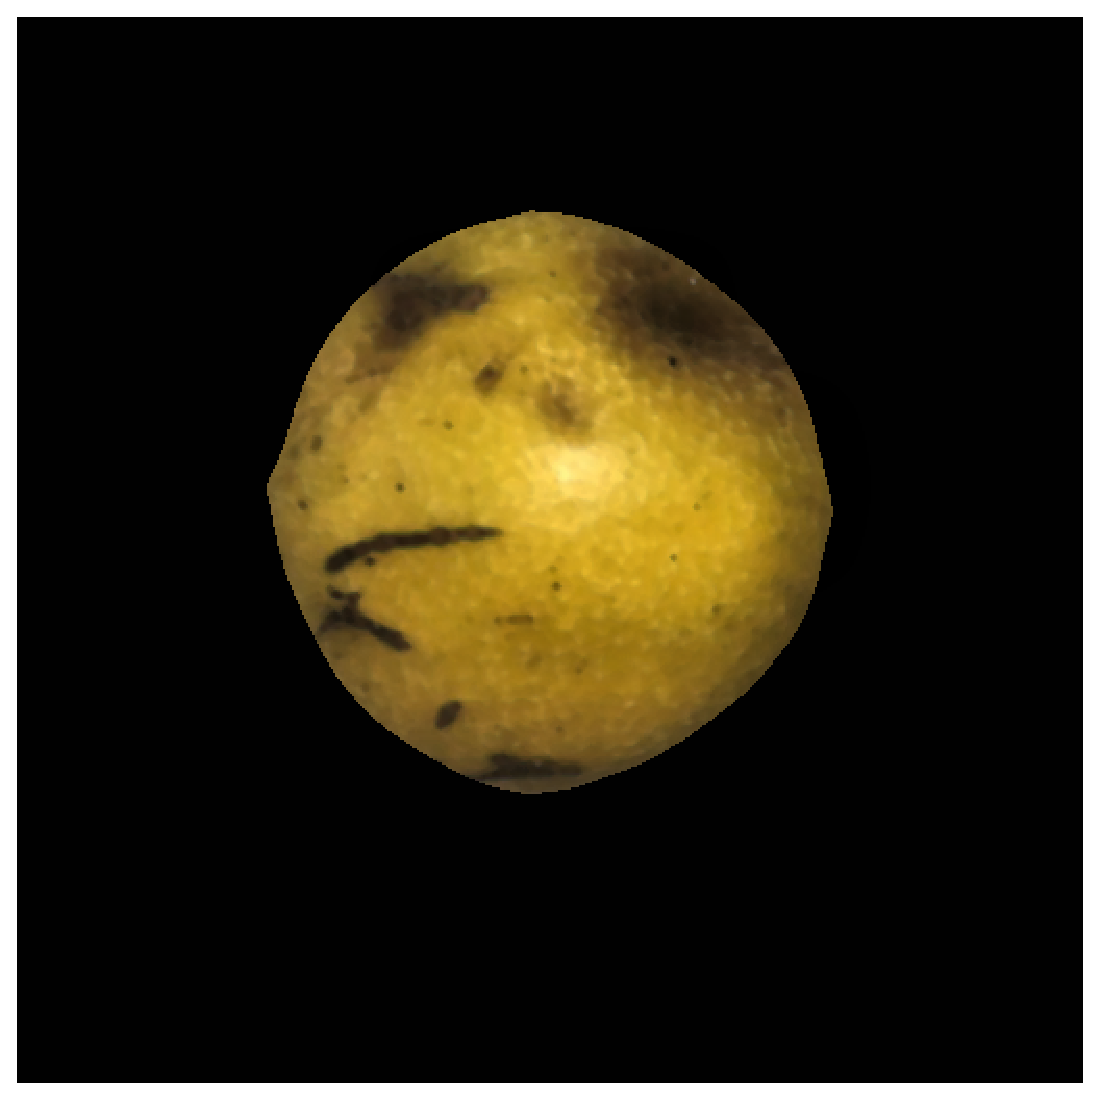
\includegraphics[width=.15\textwidth]{images/classes/abiu-medium.eps}
    }
    \subfloat[Class C]{
        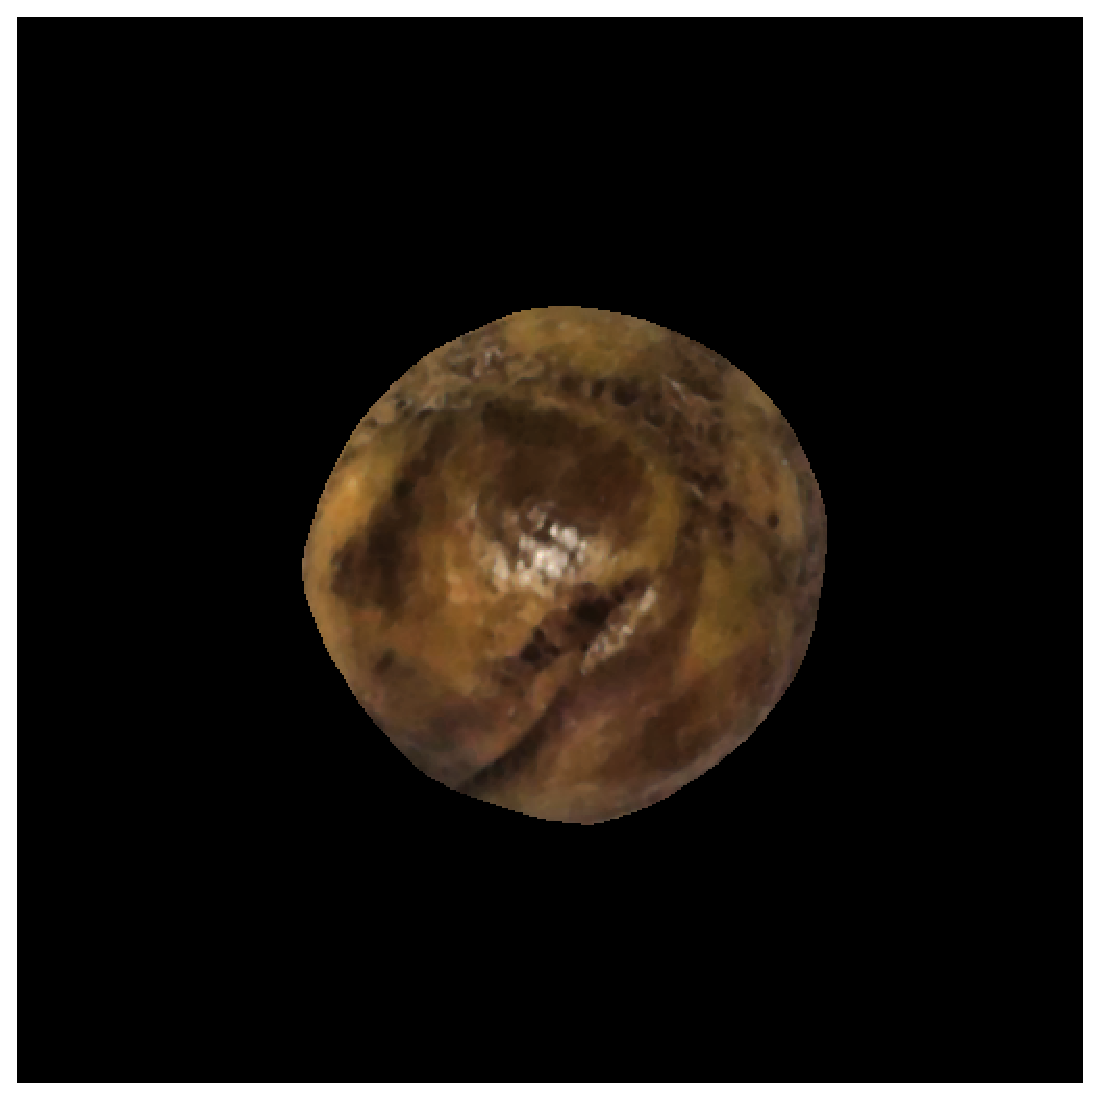
\includegraphics[width=.15\textwidth]{images/classes/abiu-bad.eps}
    }
    \caption{Samples of \textit{abius}}
    \label{fig:abiu-classes}
\end{figure}

\begin{figure}
    \centering
    \subfloat[Class A]{
        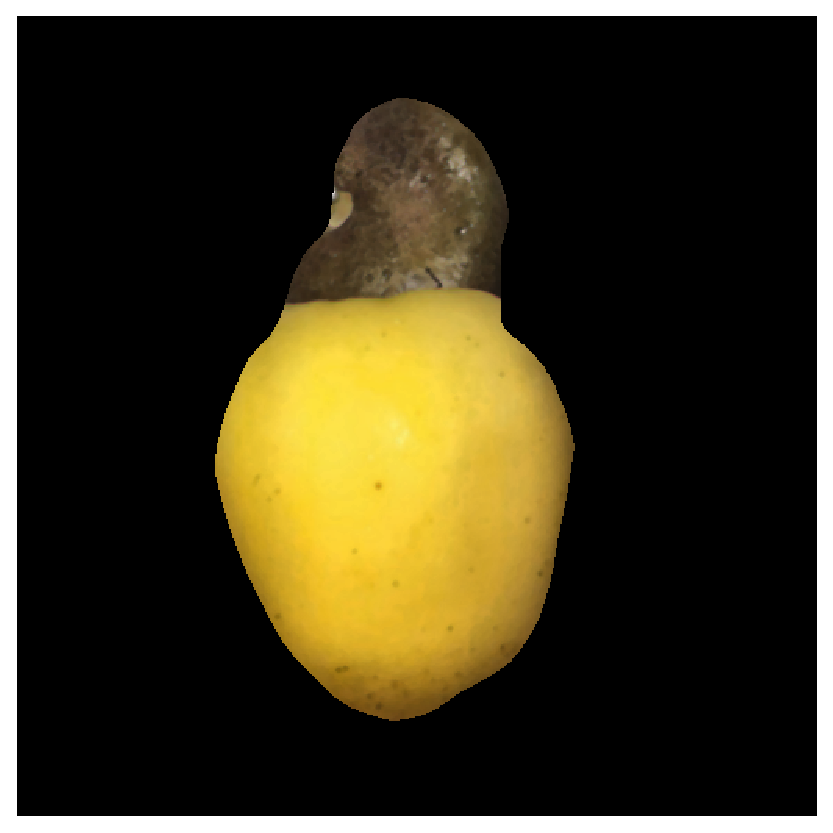
\includegraphics[width=.15\textwidth]{images/classes/caju-amarelo-good.eps}
    }
    \subfloat[Class B]{
        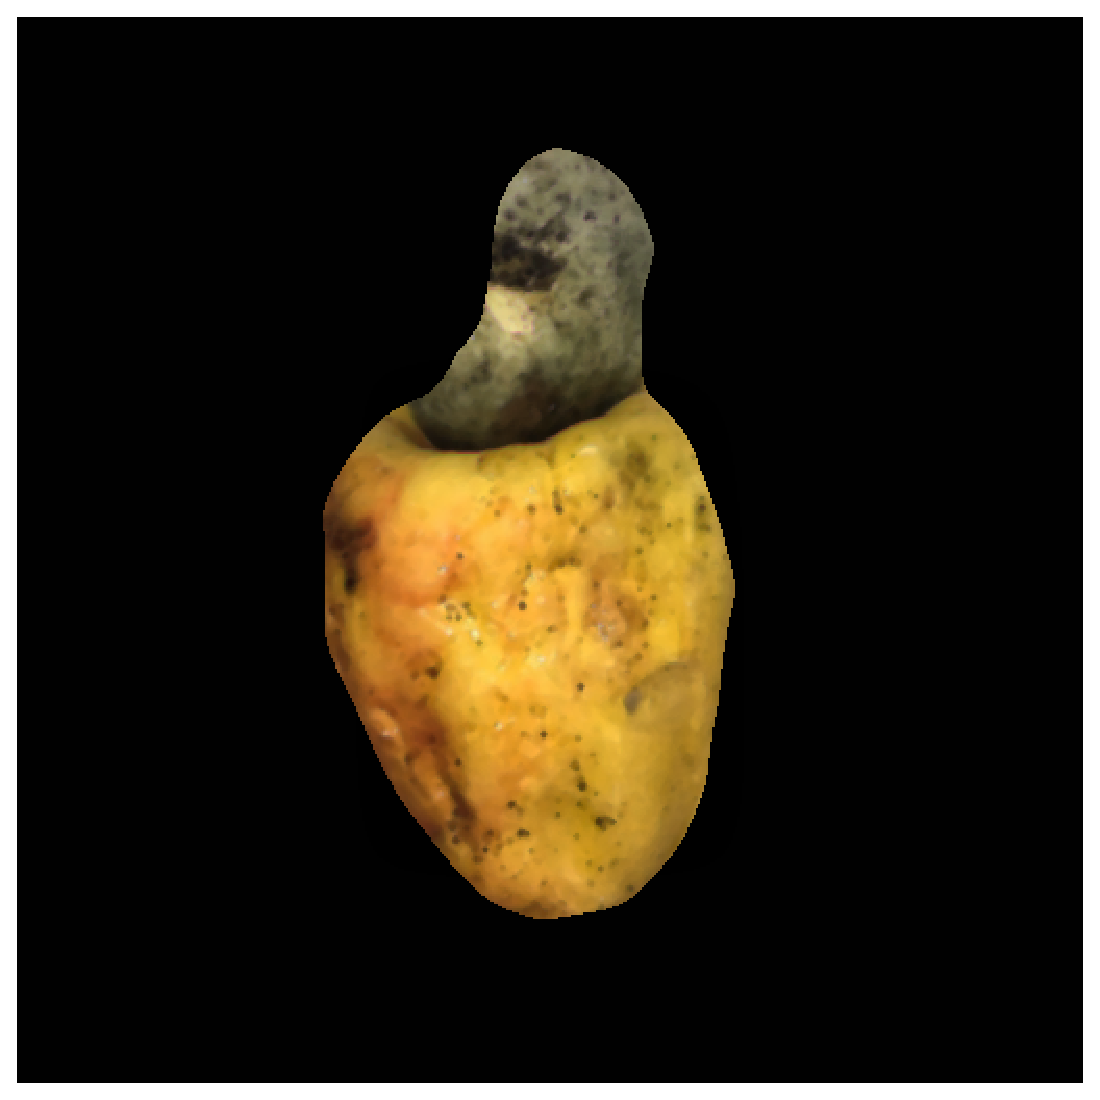
\includegraphics[width=.15\textwidth]{images/classes/caju-amarelo-medium.eps}
    }
    \subfloat[Class C]{
        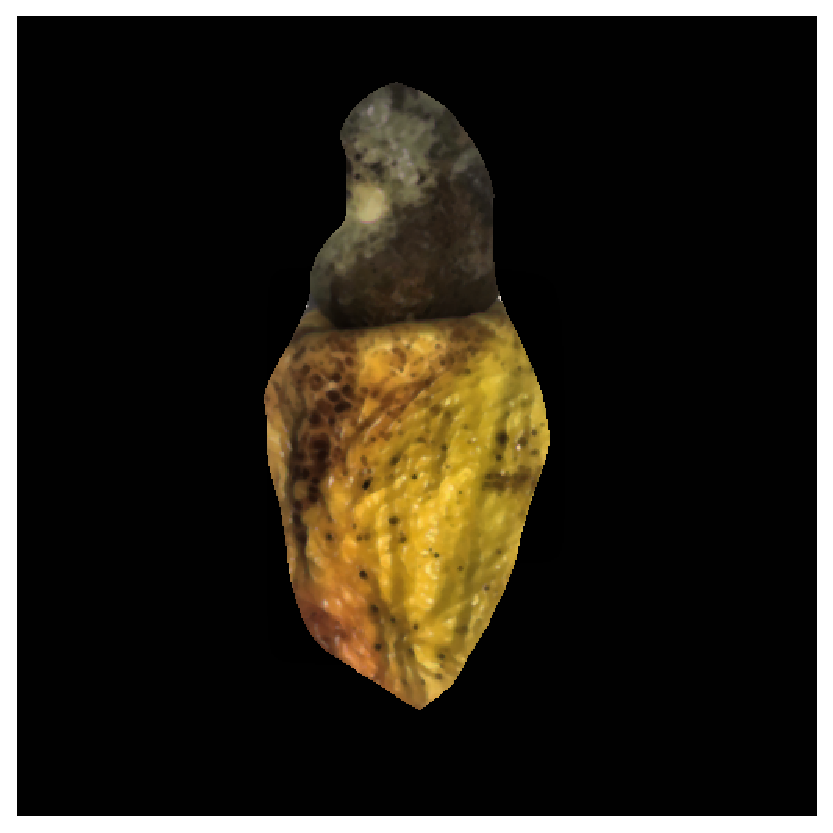
\includegraphics[width=.15\textwidth]{images/classes/caju-amarelo-bad.eps}
    }
    \caption{Samples of yellow-skinned \textit{cajus}}
    \label{fig:caju-amarelo-classes}
\end{figure}

\begin{figure}
    \centering
    \subfloat[Class A]{
        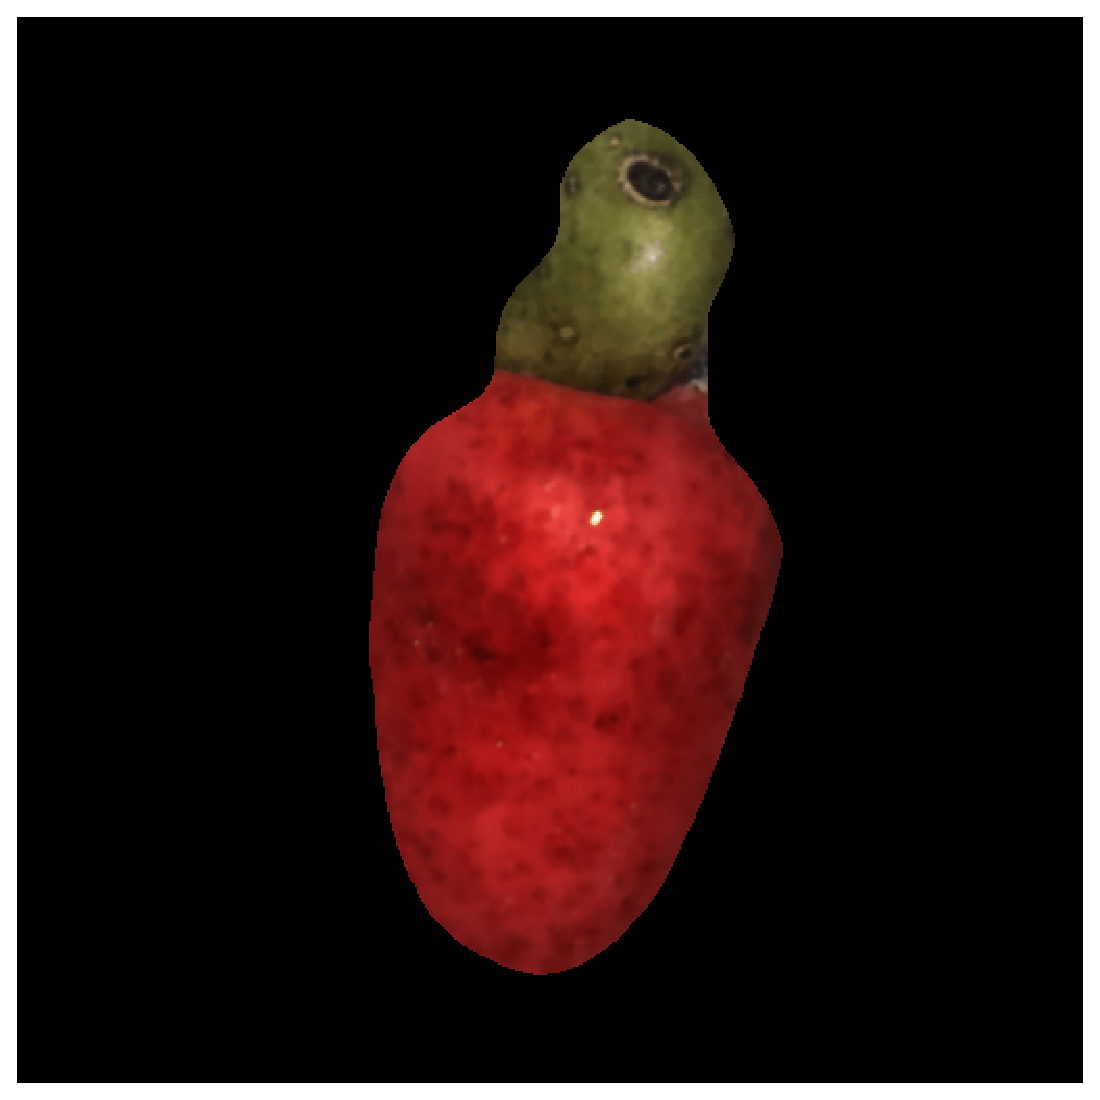
\includegraphics[width=.15\textwidth]{images/classes/caju-vermelho-good.eps}
    }
    \subfloat[Class B]{
        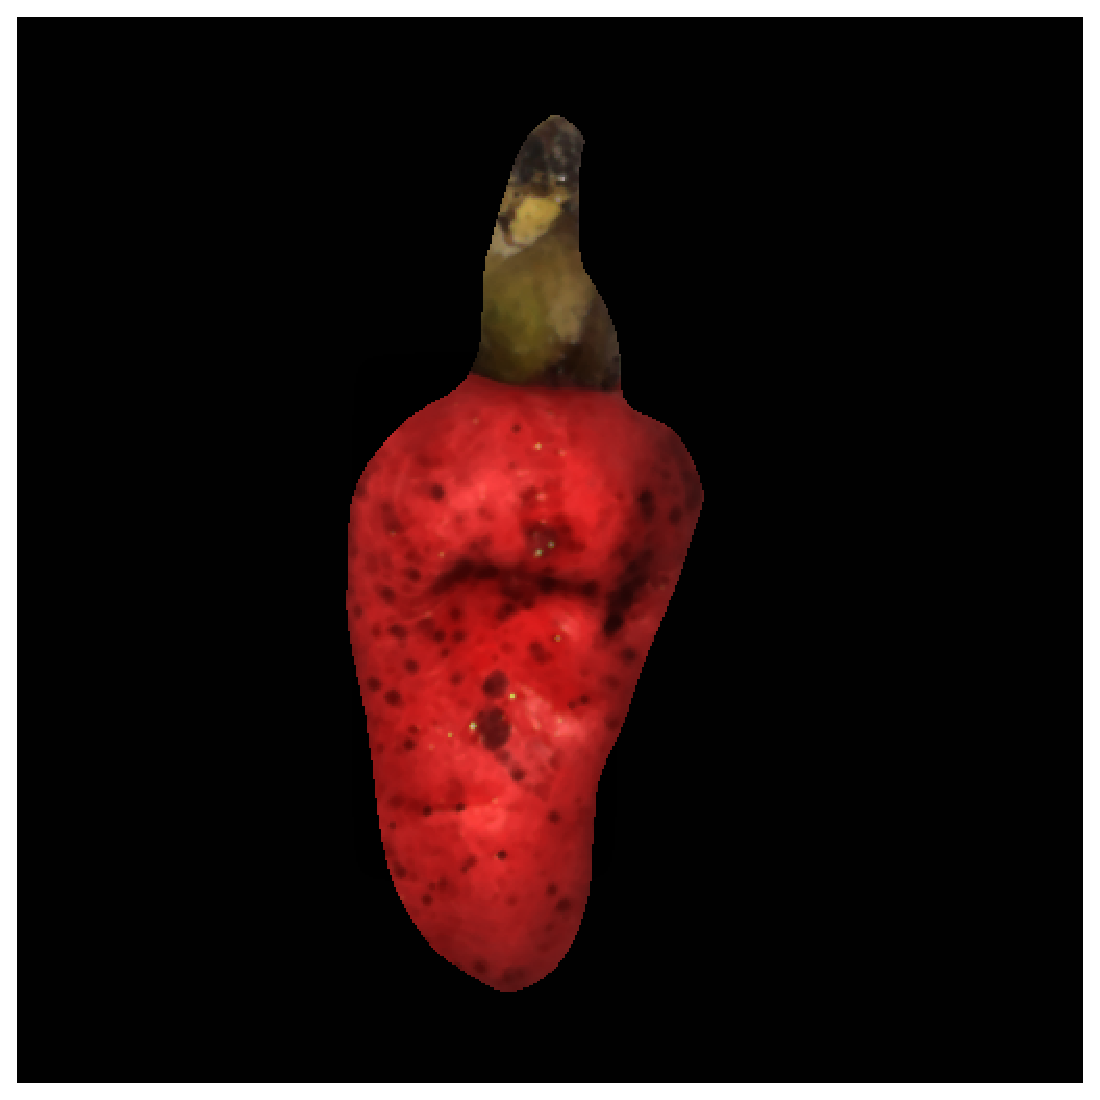
\includegraphics[width=.15\textwidth]{images/classes/caju-vermelho-medium.eps}
    }
    \subfloat[Class C]{
        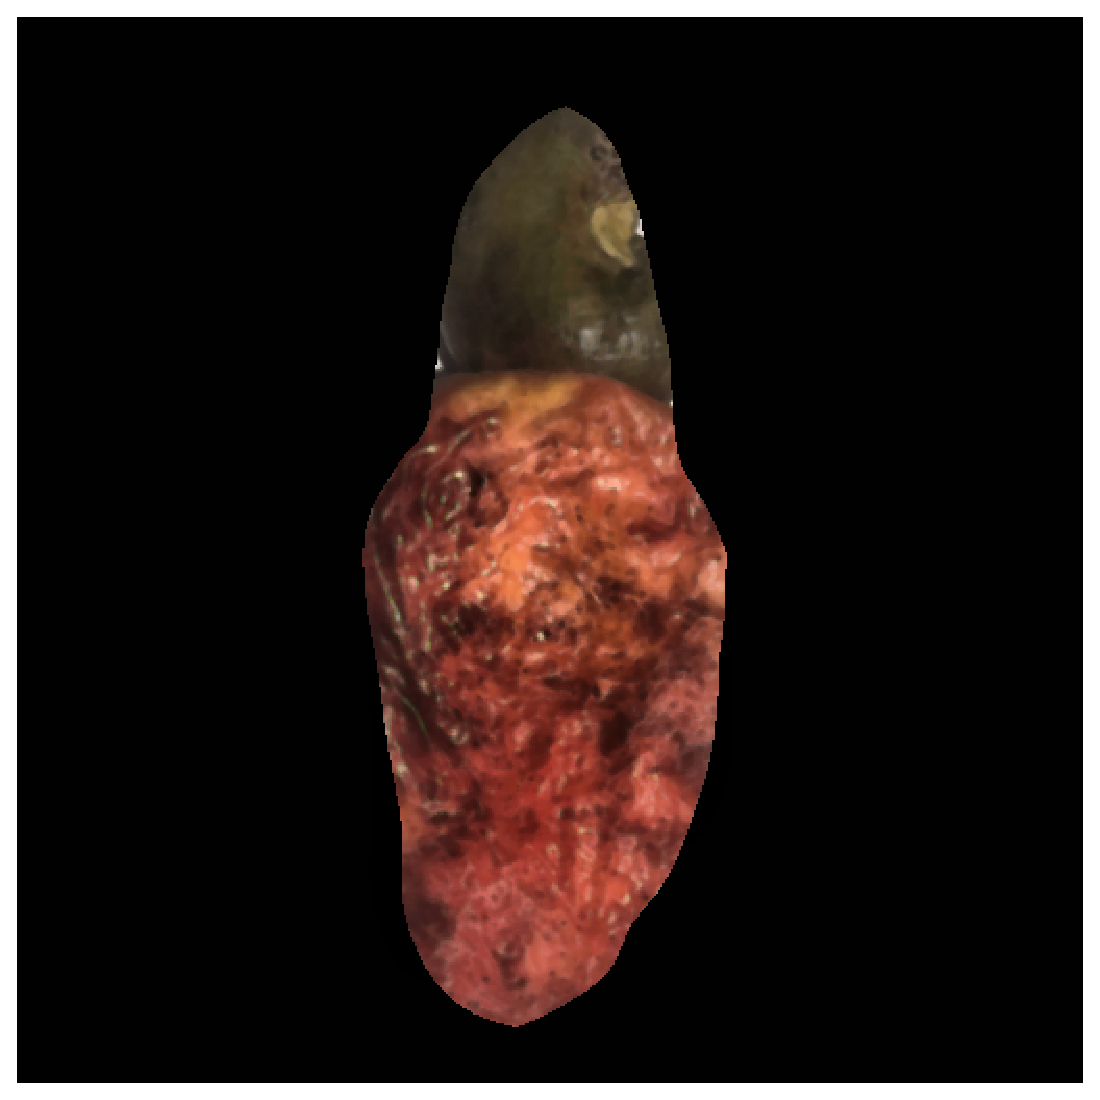
\includegraphics[width=.15\textwidth]{images/classes/caju-vermelho-bad.eps}
    }
    \caption{Samples of red-skinned \textit{cajus}}
    \label{fig:caju-vermelho-classes}
\end{figure}

\begin{figure}
    \centering
    \subfloat[Class A]{
        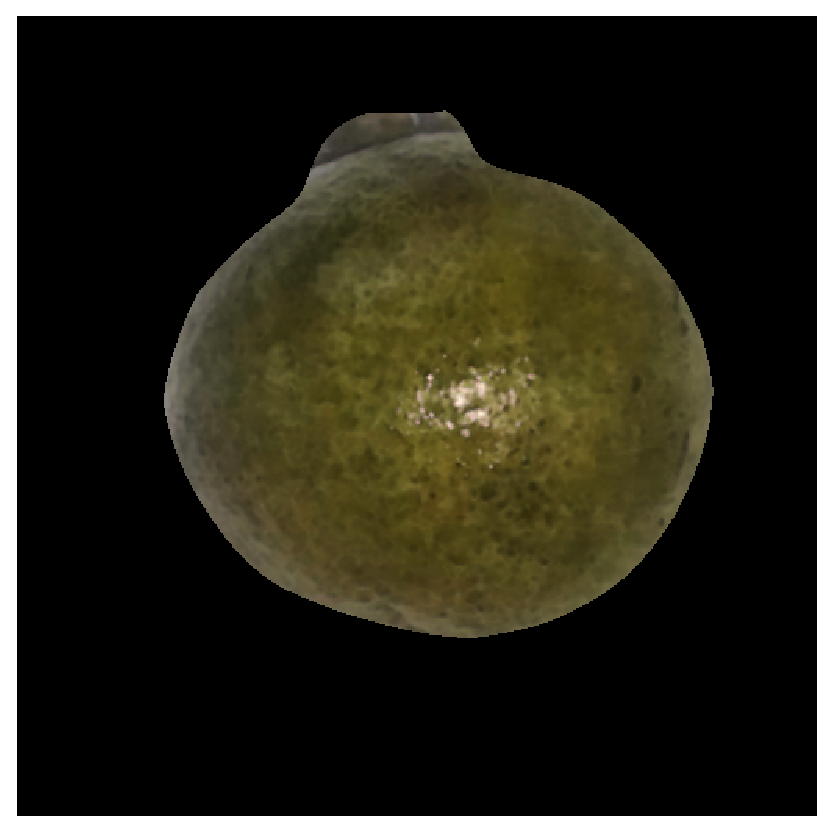
\includegraphics[width=.15\textwidth]{images/classes/gabiroba-good.eps}
    }
    \subfloat[Class B]{
        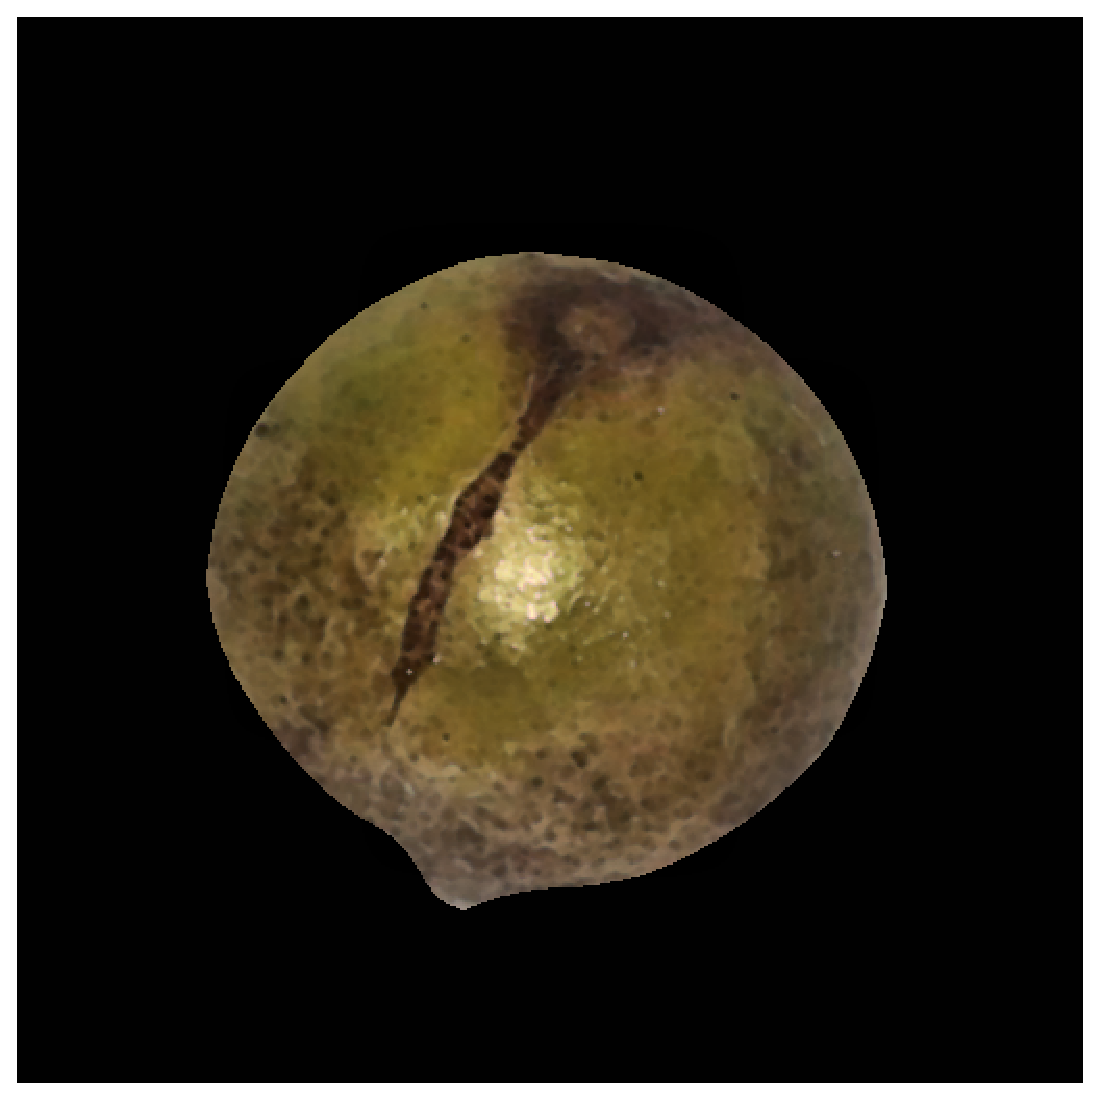
\includegraphics[width=.15\textwidth]{images/classes/gabiroba-medium.eps}
    }
    \subfloat[Class C]{
        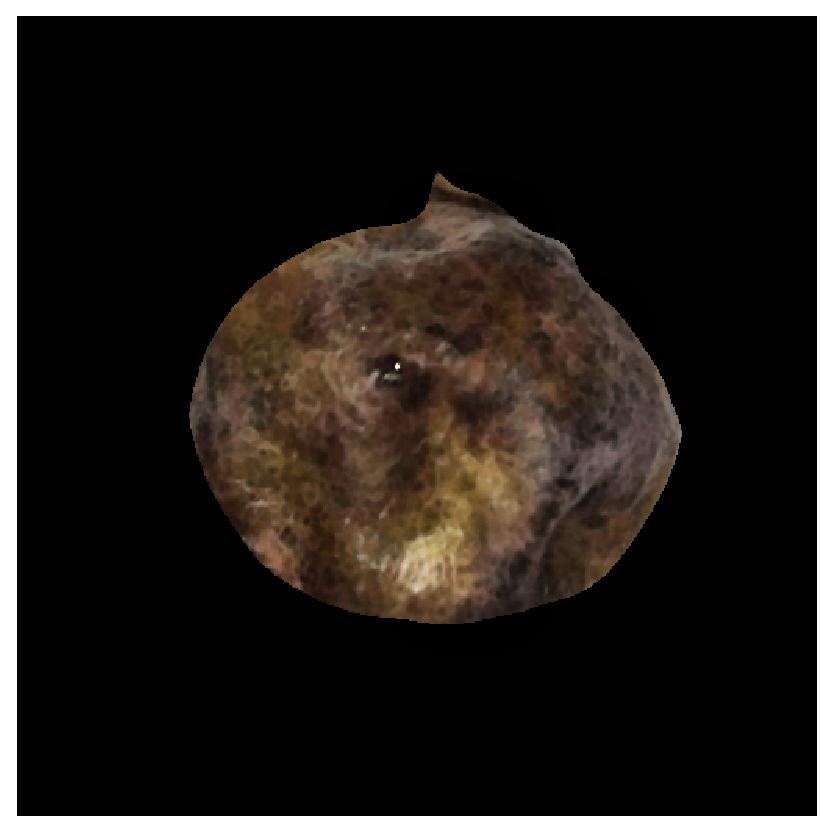
\includegraphics[width=.15\textwidth]{images/classes/gabiroba-bad.eps}
    }
    \caption{Samples of \textit{gabirobas}}
    \label{fig:gabiroba-classes}
\end{figure}

\begin{figure}
    \centering
    \subfloat[Class A]{
        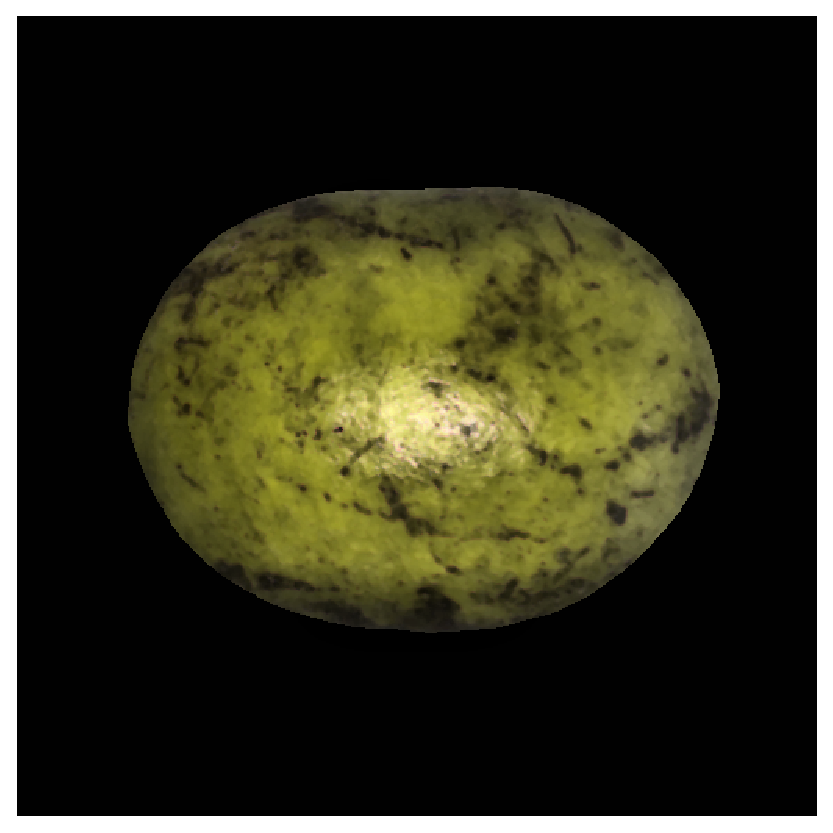
\includegraphics[width=.15\textwidth]{images/classes/pequi-good.eps}
    }
    \subfloat[Class B]{
        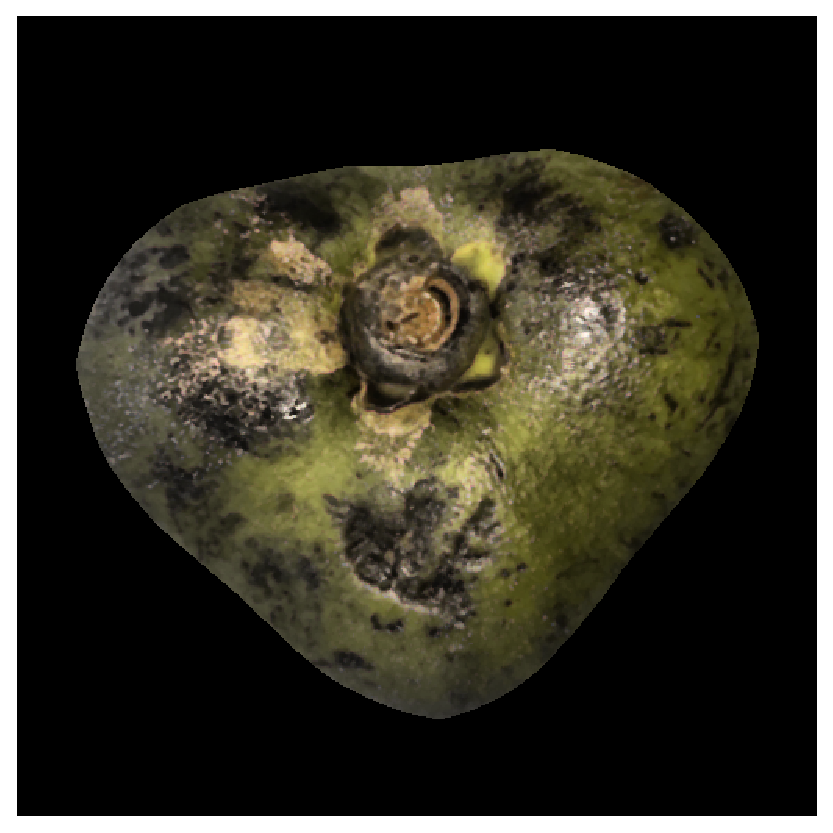
\includegraphics[width=.15\textwidth]{images/classes/pequi-medium.eps}
    }
    \subfloat[Class C]{
        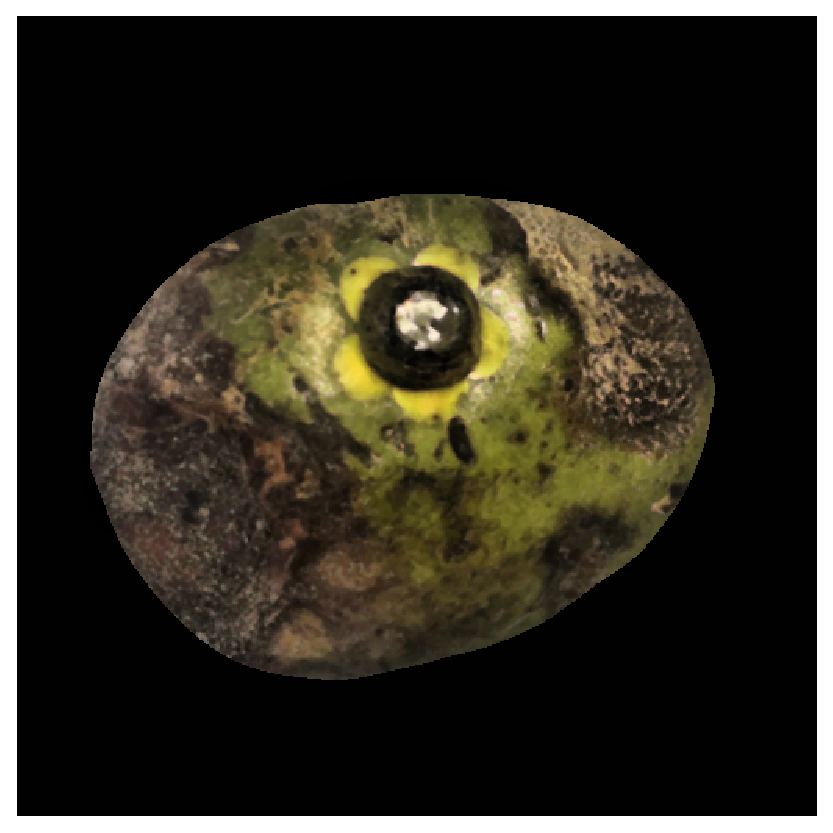
\includegraphics[width=.15\textwidth]{images/classes/pequi-bad.eps}
    }
    \caption{Samples of \textit{pequi}}
    \label{fig:pequi-classes}
\end{figure}

\begin{figure}
    \centering
    \subfloat[Class A]{
        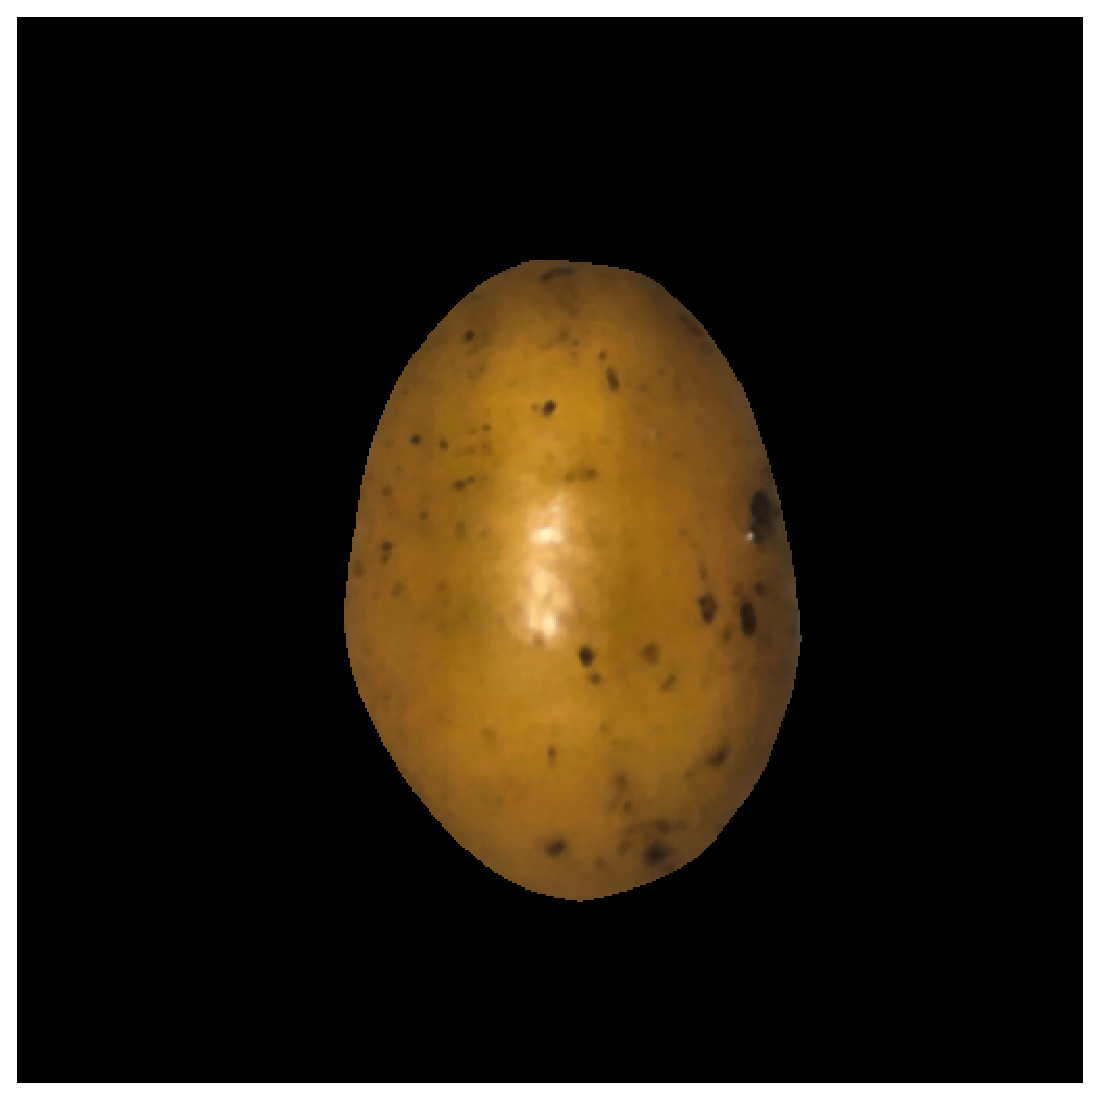
\includegraphics[width=.15\textwidth]{images/classes/siriguela-good.eps}
    }
    \subfloat[Class B]{
        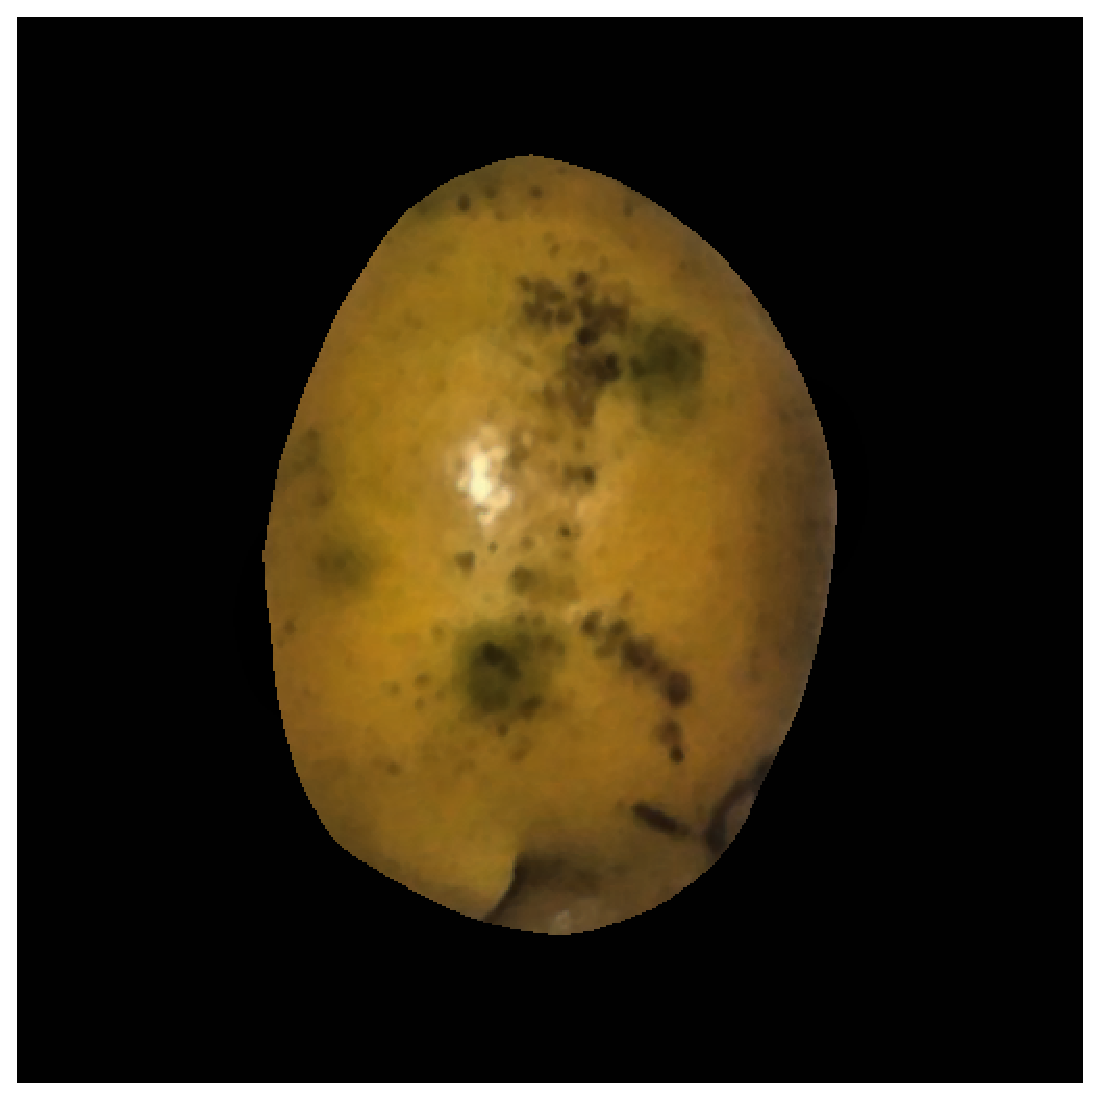
\includegraphics[width=.15\textwidth]{images/classes/siriguela-medium.eps}
    }
    \subfloat[Class C]{
        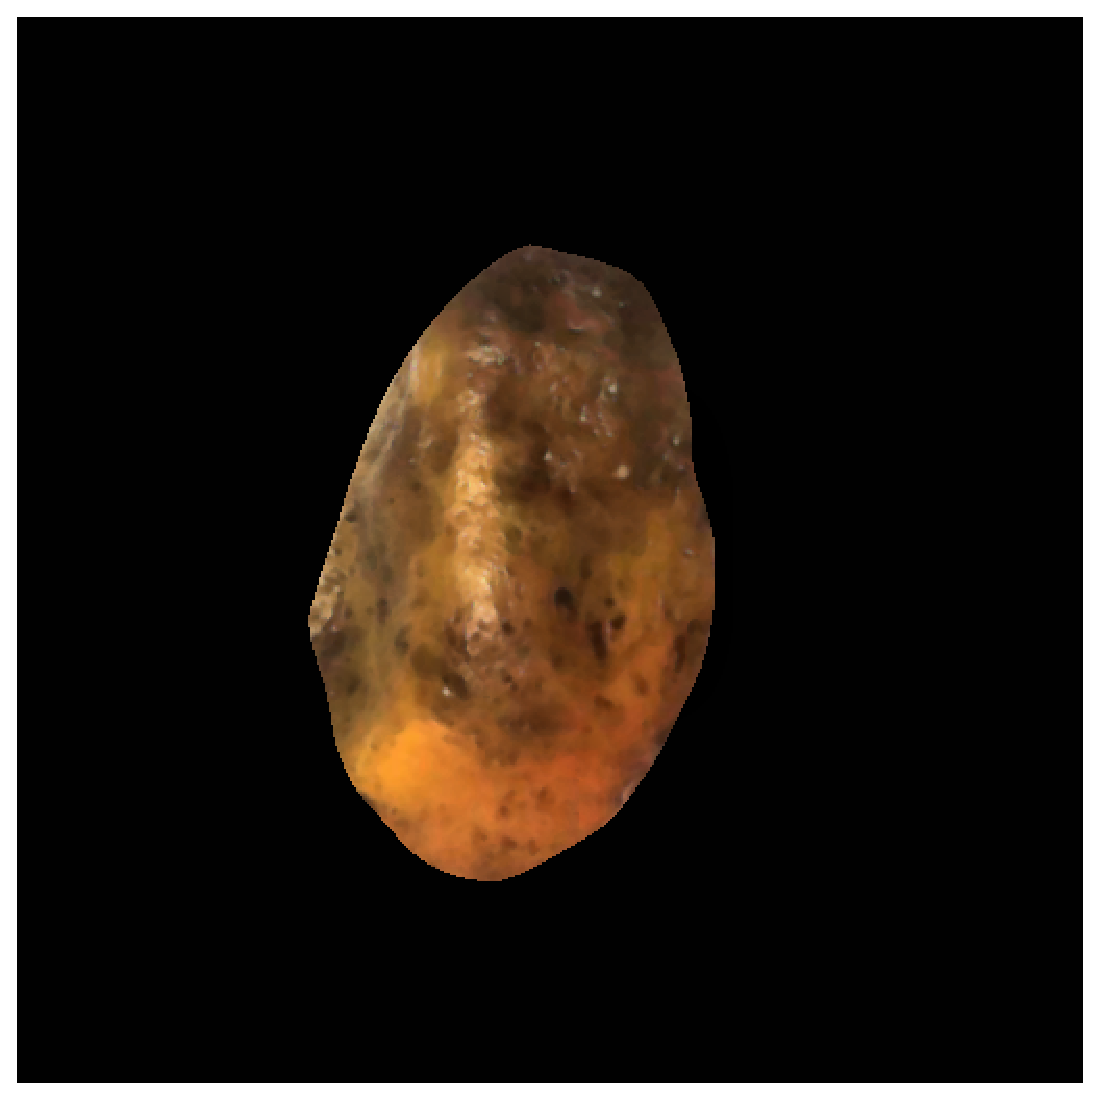
\includegraphics[width=.15\textwidth]{images/classes/siriguela-bad.eps}
    }
    \caption{Samples of \textit{siriguelas}}
    \label{fig:siriguela-classes}
\end{figure}

\end{document}